\documentclass[tikz]{standalone}
\usepackage{pgfplots}
\pgfplotsset{compat=1.15}
\usepackage{mathrsfs}
\usetikzlibrary{arrows,calc}
\usepackage{tkz-euclide}

\pagestyle{empty}

\definecolor{AngleClr}{rgb}{0,0.39215686274509803,0}
\definecolor{ShapeClr}{rgb}{0.6,0.2,0}

\begin{document}

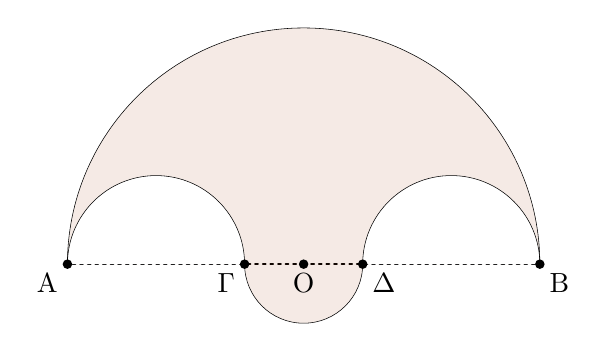
\begin{tikzpicture}[scale=.75]
\tkzSetUpLine[line width=1pt,color=black]
\tkzSetUpPoint[fill=black]

\tkzDefPoints{0/0/O,-4/0/A,4/0/B,-1/0/C,1/0/D}

\tkzDefMidPoint(A,C) \tkzGetPoint{O1}
\tkzDefMidPoint(D,B) \tkzGetPoint{O2}

\tkzDrawSegments[line width=0.75pt,color=black, dashed,dash pattern=on 1pt off 1.75pt](O,A O,B)

% \tkzDrawCircle[color=black,line width=0.5pt](O,X)

\tkzFillSector[ShapeClr,fill opacity=0.1](O,B)(A)
\tkzFillSector[white](O1,C)(A)
\tkzFillSector[white](O2,B)(D)
\tkzFillSector[ShapeClr,fill opacity=0.1](O,C)(D)

\tkzDrawArc(O,B)(A)
\tkzDrawArc(O1,C)(A)
\tkzDrawArc(O2,B)(D)
\tkzDrawArc(O,C)(D)


\tkzDrawPoints[size=3](A,B,O,C,D)
\tkzLabelPoint[below left](A){$\rm A$}
\tkzLabelPoint[below right](B){$\rm B$}
\tkzLabelPoint[below left](C){$\rm \Gamma$}
\tkzLabelPoint[below right](D){$\rm \Delta$}
\tkzLabelPoint[below](O){$\rm O$}

\end{tikzpicture}

\end{document}
